\section{sparse grid for $x^2$}
Consider multilevel grid points
$$
T_k:\quad x_i^k = ih_k,\quad h_k = 2^{-k},\quad k=0,1,2,...,J,\quad 0\le i\le 2^k.
$$
Consider linear interpolation on $T_k$:
$$
(I_k v)(x) = \sum_{i=0}^{2^k}v(x_i^k)\varphi_i^k(x).
$$
Let $v(x)=x^2$, it is easy to see that
$$
(I_0v)(x) = x.
$$
For $k\ge 1$,
\[
\begin{split}
(I_k-I_{k-1})v &= \sum_{j=1}^{2^{k-1}}[(I_k-I_{k-1})v]\varphi_{2j-1}^k(x)\\
&=\sum_{j=1}^{2^{k-1}}[v(x_{2j-1}^k)-\frac{1}{2}(v(x_{2j-2}^k)+v(x_{2j}^k))]\varphi_{2j-1}^k(x)\\
&=\sum_{j=1}^{2^{k-1}}\frac{1}{2}h_k^2[2(2j-1)^2-(2j-2)^2-(2j)^2]\varphi_{2j-1}^k(x)\\
&=-\sum_{j=1}^{2^{k-1}}4^{-k}\varphi_{2j-1}^k(x)\\
&=-4^{-k}\underbrace{\varphi_1\circ\cdots\circ\varphi_1(x)}\limits_{\varphi_k}.
\end{split}
\]

\begin{lemma}
	$$
	I_J(x^2) = x-\sum_{k=1}^J4^{-k}\varphi_k(x).
	$$
\end{lemma}
Consequently,
\[
\begin{split}
x^2 &= I_Jv + O(h_J^2) = I_0v+\sum_{k=1}^J(I_k-I_{k-1})v+O(h_J^2)\\
&=x - \sum_{k=1}^J4^{-k}\varphi_k + O(h_J^2)
\end{split}
\]



\section{sparse grid for $x^3$}

Given $(x_i,y_i),i=1,2,3,$ the quadratic interpolation function is 
\[
I(x) = y_1\frac{(x-x_2)(x-x_3)}{(x_1-x_2)(x_1-x_3)}+y_2\frac{(x-x_1)(x-x_3)}{(x_2-x_1)(x_2-x_3)}+y_3\frac{(x-x_1)(x-x_2)}{(x_3-x_1)(x_3-x_2)}.
\]
On grid 
\[T_k: x_i = i2^{-k},\quad i = 0,...,2^k,
\]
we have the piece quadratic interpolation on each $[x_i,x_{i+1}]$. Define $x_{i+\frac{1}{2}} = \frac{1}{2}(x_i+x_{i+1})$, then we have the basis function $\varphi_i^k,\varphi_{i+\frac{1}{2}}^k,\varphi_{i+1}^k$.

On grid 
\[T_{k+1}: x_i = i2^{-(k+1)},\quad i = 0,...,2^{k+1},
\]
we have the basis function $\varphi_i^{k+1},\varphi_{i+\frac{1}{4}}^{k+1},\varphi_{i+\frac{1}{2}}^{k+1}$ on $[x_i,x_{i+\frac{1}{2}}]$ and $\varphi_{i+\frac{1}{2}}^{k+1},\varphi_{i+\frac{3}{4}}^{k+1},\varphi_{i+1}^{k+1}$ on $[x_{i+\frac{1}{2}},x_{i+1}]$. The basis function $\varphi^{k+1}_i$ satisfies
\[
\varphi^{k+1}_i(x_i) = 1,\quad \varphi^{k+1}_i(x_{i-\frac{1}{4}}) = 0,\quad \varphi^{k+1}_i(x_{i+\frac{1}{4}}) = 0,
\]
and $\varphi^{k+1}_i$ is a quadratic function on $[x_{i-\frac{1}{4}},x_{i+\frac{1}{4}}],$and equal to $0$ out of $[x_{i-\frac{1}{4}},x_{i+\frac{1}{4}}].$
Then we have 
\[
\begin{split}
I_k(x^3) &= x_i^3\varphi_i^k + x_{i+{\frac{1}{2}}}^3\varphi_{i+\frac{1}{2}}^k + x_{i+1}^3\varphi_{i+1}^k\\
&=x_i^3(\varphi^{k+1}_i + \frac{3}{8}\varphi^{k+1}_{i+\frac{1}{4}}-\frac{1}{8}\varphi^{k+1}_{i+\frac{3}{4}})\\
&+x_{i+\frac{1}{2}}^3(\frac{3}{4}\varphi^{k+1}_{i+\frac{1}{4}}+\varphi^{k+1}_{i+\frac{1}{2}}+\frac{3}{4}\varphi^{k+1}_{i+\frac{3}{4}})\\
&+ x_{i+1}^3(-\frac{1}{8}\varphi_{i+\frac{1}{4}}^{k+1}+\frac{3}{8}\varphi_{i+\frac{3}{4}}^{k+1}+\varphi_{i+1}^{k+1})
\end{split}
\]
and 
\[
I_{k+1}(x^3) = x_i^3\varphi_i^{k+1} + x_{i+\frac{1}{4}}^3\varphi_{i+\frac{1}{4}}^{k+1} + x_{i+\frac{1}{2}}^3\varphi_{i+\frac{1}{2}}^{k+1} + x_{i+\frac{3}{4}}^3\varphi_{i+\frac{3}{4}}^{k+1} + x_{i+1}^3\varphi_{i+1}^{k+1}
\]
Then on $[x_i,x_{i+1}]$
\[
\begin{split}
(I_{k+1}-I_k)(x^3) &=(x^{3}_{i+\frac{1}{4}}-\frac{3}{8}x_i^3-\frac{3}{4}x_{i+\frac{1}{2}}^3+\frac{1}{8}x^3_{i+1})\varphi_{i+\frac{1}{4}}^{k+1} +(x_{i+\frac{3}{4}}^3+\frac{1}{8}x_i^3-\frac{3}{4}x_{i+\frac{1}{2}}^3-\frac{3}{8}x^3_{i+1})\varphi_{i+\frac{3}{4}}^{k+1}\\
&=3\times2^{-3k-6}(\varphi_{i+\frac{1}{4}}^{k+1}-\varphi_{i+\frac{3}{4}}^{k+1})
\end{split}
\]
where $\varphi_{i+\frac{1}{4}}^{k+1}-\varphi_{i+\frac{3}{4}}^{k+1}$ is 
\begin{center}
	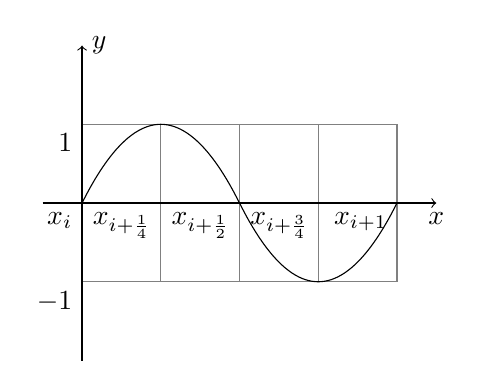
\begin{tikzpicture}[scale = 1]
	\draw[gray, step = 1cm] (0, -1) grid (4, 1);
	\draw[->] (-.5, 0) -- (4.5, 0);
	\draw[->] (0, -2) -- (0, 2);
	
	\node[anchor = north east] at (0, 0) {$ x_i $};
	\node[anchor = north east] at (1, 0) {$ x_{i+\frac{1}{4}} $};
	\node[anchor = north east] at (2, 0) {$ x_{i+\frac{1}{2}} $};
	\node[anchor = north east] at (3, 0) {$ x_{i+\frac{3}{4}} $};
	\node[anchor = north east] at (4, 0) {$ x_{i+1} $};
	\node[anchor = north east] at (0, 1) {$ 1 $};
	\node[anchor = north east] at (0, -1) {$ -1 $};
	\node[anchor = north] at (4.5, 0) {$ x $};
	\node[anchor = west] at (0, 2) {$ y $};
	
	
	\draw[domain = 0:2, smooth, variable=\x, black]
	plot ({\x}, {\x * (2-\x)})
	node[anchor = west] {};
	\draw[domain = 2:4, smooth, variable=\x, black]
	plot ({\x}, {-(4-\x) * (\x-2)})
	node[anchor = west] {};
	\end{tikzpicture}
\end{center}

We sum all the function on $[0,1]$,
\[
(I_{k+1}-I_k)(x^3) = 3\times2^{-3k-6}\sum_{i=0}^{2^k-1}(\varphi_{i+\frac{1}{4}}^{k+1} - \varphi_{i+\frac{3}{4}}^{k+1})
\]


\section{2D sparse grid for $xy$}
Consider the uniform gird $[0,1]^2$, and we define the grid
\[
T_k:(x_i,y_j),\quad x_i = ih,y_j = jh,\quad h = 2^{-k}
\]
$I_k$ is the piece linear interpolation operator which satisfies 
\[
(I_k f)(x_i,y_j) = f(x_i,y_j)
\]
We consider the grid $T_k$ and $T_{k-1}$. 
\begin{itemize}
	\item The basis functions on $T_{k-1}$ are $\varphi_1^{k-1},\varphi_2^{k-1},\varphi_3^{k-1}$.
	\item  The basis functions on refine grid $T_k$ are $\varphi_i^k,i=1,..,6$.
\end{itemize}
\begin{center}
	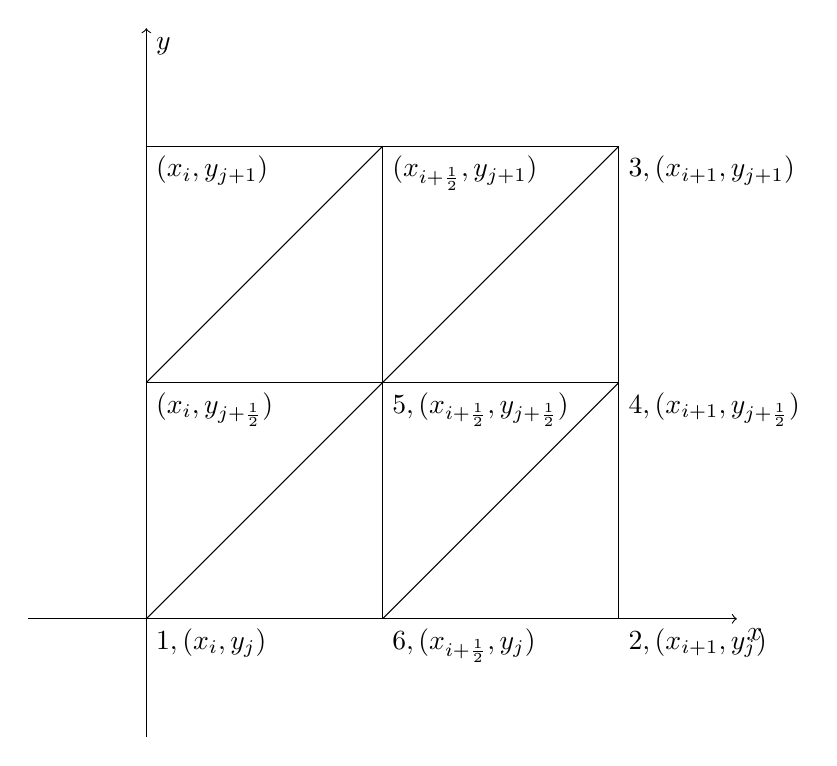
\begin{tikzpicture}[scale = 3 ]
	\draw[gray, step = 1cm] (0, 0) grid (2, 2);
	\draw[->] (-.5, 0) -- (2.5, 0);
	\draw[->] (0, -.5) -- (0, 2.5);
	\node[anchor = north west] at (0, 0) {$1, (x_i,y_j) $};
	\node[anchor = north west] at (2.5, 0) {$ x $};
	\node[anchor = north west] at (0, 2.5) {$ y $};
	\node[anchor = north west] at (1,0) {$6,(x_{i+\frac{1}{2}},y_j)$};
	\node[anchor = north west] at (2,0) {$2,(x_{i+1},y_j)$};
	\node[anchor = north west] at (0,1) {$(x_{i},y_{j+\frac{1}{2}})$};
	\node[anchor = north west] at (1,1) {$5,(x_{i+\frac{1}{2}},y_{j+\frac{1}{2}})$};
	\node[anchor = north west] at (2,1) {$4,(x_{i+1},y_{j+\frac{1}{2}})$};
	\node[anchor = north west] at (0,2) {$(x_{i},y_{j+1})$};
	\node[anchor = north west] at (1,2) {$(x_{i+\frac{1}{2}},y_{j+1})$};
	\node[anchor = north west] at (2,2) {$3,(x_{i+1},y_{j+1})$};
	
	\draw (0,0) -- (0,2);
	\draw (0,2) -- (2,2);
	\draw (2,2) -- (2,0);
	\draw (2,0) -- (0,0);
	\draw (0,0) -- (2,2);
	\draw (0,1) -- (1,2);
	\draw (1,0) -- (2,1);
	\draw (1,0) -- (1,2);
	\draw (0,1) -- (2,1);
	\end{tikzpicture}
\end{center}
\[
\begin{split}
I_{k-1}(xy) &= x_iy_j\varphi^{k-1}_1 + x_{i+1}y_j\varphi^{k-1}_2 + x_{i+1}y_{j+1}\varphi^{k-1}_3\\
&=x_iy_j(\varphi^k_1 + \frac{1}{2}(\varphi^k_5+\varphi^k_6)) + x_{i+1}y_j(\varphi^k_2 + \frac{1}{2}(\varphi^k_4+\varphi^k_6))\\
&+x_{i+1}y_{j+1}(\varphi^k_3+\frac{1}{2}(\varphi^k_4+\varphi^k_5))\\
&=x_iy_j\varphi^k_1 + x_{i+1}y_j\varphi^k_2+x_{i+1}y_{j+1}\varphi^k_3+\frac{1}{2}(x_{i+1}y_j+x_{i+1}y_{j+1})\varphi^k_4\\
&+\frac{1}{2}(x_{i}y_j+x_{i+1}y_{j+1})\varphi^k_5+\frac{1}{2}(x_{i}y_j+x_{i+1}y_{i})\varphi^k_6\\
&=x_iy_j\varphi^k_1 + x_{i+1}y_j\varphi^k_2+x_{i+1}y_{j+1}\varphi^k_3+x_{i+1}y_{j+\frac{1}{2}}\varphi^k_4\\
&+\frac{1}{2}(x_{i}y_j+x_{i+1}y_{j+1})\varphi^k_5+x_{i+\frac{1}{2}}y_j\varphi^k_6\\
I_k(xy) & = x_iy_j\varphi^k_1+x_{i+1}y_j\varphi^k_2+x_{i+1}y_{j+1}\varphi^k_3+x_{i+1}y_{j+\frac{1}{2}}\varphi^k_4 \\
&+x_{i+\frac{1}{2}}y_{j+\frac{1}{2}}\varphi^k_5 + x_{i+\frac{1}{2}}y_j\varphi^k_6
\end{split}
\]

Then,
\[
(I_k - I_{k-1})(xy) = (x_{i+\frac{1}{2}}y_{j+\frac{1}{2}}-\frac{1}{2}(x_{i}y_j+x_{i+1}y_{j+1}))\varphi^k_5 = -\frac{h^2}{4}\varphi_5^k
\]
The error is uniform! which is the basis function on each rectangle $[x_i,x_{i+1}]\times [y_j,y_{j+1}]$ and 
\[
\varphi_5^k(x_{i+\frac{1}{2}},y_{j+\frac{1}{2}}) = 1
\]


\section{Spectral approximation properties of ReLU DNN}
Here we will talk about how to use ReLU DNN to approximate polynomials
and then achieve the ``spectral" accuracy for analytical functions.
The main results can be found in \cite{yarotsky2017error},
\cite{wang2018exponential}. Some related works are
\cite{liang2016why,lu2017expressive}

First, we will introduce the following notation
\begin{itemize}
\item $x=(x_1,\ldots,x_d)$.
\item Colon notation for subscript: let $\{x_{m:n}\} = \{x_i:i = m,m+1,...,n\}$ and $\{x_{m_1:n_1,m_2:n_2}\}= \{x_{i,j}:i = m_1,...,n_1,j = m_2,...,n_2\}.$ 
\item Linear combination: denote $y\in \mathcal L(x_1,...,x_d)$ if
  there exist $\beta_i\in \mathbb{R},i=1,...,d,$ such that $y =
  \beta_0+\beta_1x_1+\cdots+\beta_d x_d$.
\item Linear combination with ReLU activation: denote $\tilde{y}\in
  \tilde{\mathcal L}(x_1,...,x_d)$ if there exists $y\in
  \mathcal{L}(x_1,...,x_d)$ and $\tilde{y} = \mbox{ReLU}(y) =
  \max(y,0).$
\item $\tilde {\mathcal L} =\sigma\circ\mathcal L$
\end{itemize}
\begin{definition}
Given a function $f(x)$, if there exist variables $\{y_{1:L,1:M}\}$ such that 
\begin{equation}
y_{1,m}\in \tilde{\mathcal L}(x),\quad y_{l+1,m} \in \tilde{\mathcal L}(x,y_{l,1:M}),\quad f\in\mathcal{L}(x,y_{1:L,1:M}),
\end{equation}\label{def:netclass}
where $m=1,...,M,l=1,...,L-1$, then $f$ is said to be in the neural nets class $\mathcal{F}_{L,M}(\mathbb{R}^d)$, and $\{y_{1:L,1:M}\}$ is called a set of hidden variables of $f$. 
\end{definition}
\newpage
%\begin{properties}
\begin{proposition}
A function $f\in \mathcal F_{L,M}(\mathbb R^d)$ can be represented by a ReLU network with depth $L+1$ and width $M+d+1$.
\end{proposition}
%\end{properties}
\begin{proof}
Let $\{y_{1:L}\}$ be the hidden variables of $f$ that satisfies (\ref{def:netclass}), where
$$
f = \alpha_0 + \sum_{i=1}^d \alpha_ix_i+\sum_{l=1}^L\sum_{m=1}^M \beta_{l,m}y_{l,m}.
$$
$$
h\leftarrow (y,ex^T), e=(1,\ldots 1)^T.
$$
Consider the following variables $\{h_{1:L,1:M}\}$:
$$
h_{l,1:M} = y_{l,1:M}, \quad h_{l,M+1:M+d} = x_{1:d}
$$
for $l = 1,...,L,$ and
$$
h_{1,M+d+1} = \alpha_0 + \sum_{i=1}^d\alpha_ix_i,\quad h_{l+1,M+d+1} =h_{l,M+d+1} + \sum_{m=1}^M\beta_{l,m}h_{l,m}
$$
for $l=1,...,L-1$. One can see that $h_{1,m}\in \tilde{\mathcal L}(x),h_{l+1,m}\in \tilde{L}(h_{l,1:M+d+1}),m = 1,...,M+d+1,l = 1,...,L-1,$ and $f\in \mathcal{L}(h_{L,1:M+d+1}),$ which is a representation of a standard neural net.
\end{proof}

%\begin{properties}
\begin{proposition}\label{prop:net class}
(Addition and composition of neural net class $\mathcal F_{L,M}$)
\begin{itemize}
\item[1]
$$
\mathcal F_{L_1,M} + \mathcal{F}_{L_2,M} \subseteq \mathcal{F}_{L_1+L_2,M},
$$
i.e. if $f_1\in \mathcal F_{L_1,M}(\mathbb{R}^d)$ and $f_2\in \mathcal{F}_{L_2,M}(\mathbb{R}^d),$ then $f_1+f_2\in\mathcal{F}_{L_1+L_2,M}(\mathbb{R}^d)$.
\item[2]
$$
\mathcal F_{L_2,M}\circ \mathcal F_{L_1,M+1} \subseteq \mathcal F_{L_1+L_2,M+1}.
$$ 
i.e. if $f_1(x)\in \mathcal{F}_{L_1,M+1}(\mathbb{R}^d)$ and $f_2(x_0,x)\in \mathcal{F}_{L_2,M}(\mathbb{R}^{d+1}),$ then 
$$
f_2(f_1(x),x)\in \mathcal{F}_{L_1+L_2,M+1}(\mathbb{R}^d).
$$
\end{itemize}
\end{proposition}
%\end{properties}

\newpage
\begin{proof}
For the addition property, denote the hidden variables of $f_1$ and $f_2$ as $\{y_{1:L_1,1:M}^{(1)}\}$ and $\{y_{1:L_2,1:M}^{(2)}\}$. 
So we have 
\[
f_1 = \alpha_0^1 + \sum_{i=1}^d \alpha^1_ix_i+\sum_{l=1}^L\sum_{m=1}^M \beta^1_{l,m}y^{(1)}_{l,m}
\]
\[
f_2 = \alpha_0^2 + \sum_{i=1}^d \alpha^2_ix_i+\sum_{l=1}^L\sum_{m=1}^M \beta^2_{l,m}y^{(2)}_{l,m}
\]
\[
f_1+f_2 = \alpha_0^1 + \alpha_0^2 + \sum_{i=1}^d (\alpha_i^1+\alpha_i^2)x_i + \sum_{l=1}^L\sum_{m=1}^M \beta^1_{l,m}y^{(1)}_{l,m} +\sum_{l=1}^L\sum_{m=1}^M \beta^2_{l,m}y^{(2)}_{l,m}
\]
$$
y^{(1)}_{1,1:M} = \sigma\circ \mathcal{L}(x),y^{(1)}_{2,1:M} = \sigma\circ \mathcal L(x,y^{(1)}_{1,1:M}),\cdots,y^{(1)}_{L_1,1:M}=\sigma\circ \mathcal L(x,y^{(1)}_{L_1-1,1:M}),
$$
$$
y^{(2)}_{1,1:M} = \sigma\circ \mathcal{L}(x) =\sigma(\mathcal L(x)+\bm 0\cdot y^{(1)}_{L_1,1:M}) = \sigma\circ \mathcal{L}(x,y^{(1)}_{L_1,1:M})
$$
$$
y^{(2)}_{2,1:M} = \sigma\circ \mathcal L(x,y^{(2)}_{1,1:M}),\cdots,y^{(2)}_{L_2,1:M}=\sigma\circ \mathcal L(x,y^{(2)}_{L_2-1,1:M}),
$$
so $f_1 + f_2 \in \mathcal{F}_{L_1+L_2,M}$
Let
$$
y_{1:L_1,1:M} = y_{1:L_1,1:M}^{(1)},\quad y_{L_1+1:L_1+L_2,1:M} = y_{1:L_2,1:M}^{(2)}. 
$$
By definition, $\{y_{1:L_1+L_2,1:M}\}$ is a set of hidden variables of $f_1+f_2$. Thus $f_1+f_2\in \mathcal F_{L_1+L_2,M}.$

For the composition property, let the hidden variables of $f_1$ and $f_1$ as $\{y_{1:L_1,1:M+1}^{(1)}\}$ and $\{y_{1:L_2,1:M}^{(2)}\}$. Let
$$
y_{1:L_1,1:M+1} = y_{1:L_1,1:M+1}^{(1)},\quad y_{L_1+1:L_1+L_2,1:M} = y_{1:L_2,1:M}^{(2)},
$$
$$
y_{L_1+1,M+1} =\cdots= y_{L_1+L_2,M+1} = f_1(x).
$$
One can see that $\{y_{1:L_1+L_2,1:M+1}\}$ is a set of hidden variables of $f_2(f_1(\bm x),\bm x)$, thus the composition property holds.
\end{proof}

\begin{definition}
Given a continuous function $\varphi(\bm{x}),\bm{x} \in [-1,1]^d$ and a continuous function class $\mathcal F([-1,1]^d),$ define the $L^\infty$ distance
$$
\mbox{dist} (\varphi,\mathcal F) = \inf_{f\in \mathcal F} \max_{\bm x \in [-1,1]^d} |\varphi(\bm{x}) - f(\bm{x})|.
$$
\end{definition}

%\begin{properties}
\begin{proposition}\label{prop:dis}
(Addition and composition properties for distance function)
\begin{itemize}
\item[1] Let $\varphi_1$ and $\varphi_2$ be continuous functions. Let $\mathcal F_{1}$ and $\mathcal F_2$ be two continuous function classes, then 
$$
\mbox{dist}(\alpha_{1}\varphi_1+\alpha_{2}\varphi_2,\mathcal{F}_1+\mathcal F_2)\le |\alpha_1|\mbox{dist}(\varphi_1,\mathcal F_1) + |\alpha_2|\mbox{dist}(\varphi_2,\mathcal F_2),
$$
where $\alpha_1$ and $\alpha_2$ are two real numbers.
\item[2] Assume that $\varphi_1(\bm x) = \varphi_1(x_1,...,x_d),\varphi_2(y,\bm x) = \varphi_2(y,x_1,...,x_d)$ satisfy $\varphi_1([-1,1]^d)\subseteq[-1,1]$. Let $\mathcal F_1([-1,1]^d),\mathcal F_2([-1,1]^{d+1})$ be two continuous function classes, then
$$
\mbox{dist}(\varphi_2(\varphi_1(\bm x),\bm x),\mathcal F_2\circ \mathcal F_1)\le L_{\varphi_2}\mbox{dist}(\varphi_1,\mathcal F_1) +\mbox{dist}(\varphi_2,\mathcal F_2)
$$
where $L_{\varphi_2}$ is the Lipschitz norm of $\varphi_2$ with respect to $y$.
\end{itemize}
\end{proposition}
%\end{properties}
\begin{proof}
The additional property obviously holds. Now we prove the composition property. For any $f_1\in\mathcal F_1,f_2\in \mathcal F_2$, one has
\[
\begin{split}
|\varphi_2(\varphi_1(\bm x),\bm x) - f_2(f_1(\bm x),\bm x)|&\le |\varphi_2(\varphi_1(\bm x),\bm x) - \varphi_2(f_1(\bm x),\bm x)|+|\varphi_2(f_1(\bm x),\bm x)-f_2(f_1(\bm x),\bm x)|\\
& \le L_{\varphi_2} ||\varphi_1(\bm x) -f_1(\bm x)||_\infty +||\varphi_2(y,\bm x) - f_2(y,\bm x)||_\infty
\end{split}
\]
Take $f_1^* = \argmin_f ||\varphi_1(\bm x) - f(\bm x)||_\infty$ and $f_2^* = \argmin_f ||\varphi_2(y,\bm x) - f(y,\bm x)||_\infty$, then it is proved.
\end{proof}

\begin{lemma}\label{lem:xsquare}
The function $\varphi(x) = x^2,x\in [-1,1]$ can be approximated by deep neural nets with an exponential convergence rate:
$$
\mbox{dist}(x^2,\mathcal{F}_{L,2}([-1,1]))\le 2^{-2L}.
$$
\end{lemma}
\begin{proof}
Consider the function
$$
g(y) = \left\{\begin{split}
	&2y,&\quad 0\le y<1/2,\\
	&2(1-y),&\quad 1/2\le y\le 1,
	\end{split}\right.
$$
then 
\begin{equation}\label{func:g}
g(y) = 2y -4\mbox{ReLU}(y-1/2)
\end{equation}
in $[0,1]$. Define the hidden variables $\{y_{1:L,1:2}\}$ as follows:
\[
\begin{split}
 y_{1,1} = \mbox{ReLU}(x),&\quad y_{1,2}=\mbox{ReLU}(-x),\\
 y_{2,1} = \mbox{ReLU}(y_{1,1}+y_{1,2}),&\quad y_{2,2} = \mbox{ReLU}(y_{1,1}+y_{1,2}-1/2),\\
 y_{2,1} = \mbox{ReLU}(|x|),&\quad y_{2,2} = \mbox{ReLU}(|x|-1/2),\\
 y_{l+1,1} = \mbox{ReLU}(2y_{l,1}-4y_{l,2}),&\quad y_{l+1,2} = \mbox{ReLU}(2y_{l,1}-4y_{l,2}-1/2)\\
\end{split}
\]
for $l = 2,3,...,L-1$. Using induction, one can see that $|x| = y_{1,1}+y_{1,2}$ and 
\begin{equation}\label{func:glinduction}
g_l(|x|)=\underbrace{g\circ g\circ \cdots \circ g}_{l}(|x|) = 2y_{l+1,1}-4y_{l+1,2},\quad l=1,...,L-1,
\end{equation} 
for $x\in [-1,1]$. i.e.
\[
\begin{split}
g_l(|x|) &= g\left(g_{l-1}(|x|)\right)\\
         &= g(2y_{l,1}-4y_{l,2})\qquad (\mbox{Eq~(\ref{func:g})})\\
         &= 2(2y_{l,1}-4y_{l,2}) - 4\mbox{ReLU}(2y_{l,1}-4y_{l,2}-1/2)\qquad (g_{l-1}(|x|)\ge 0~\mbox{if}~x\in[0,1])\\
         &= 2\mbox{ReLU}(2y_{l,1}-4y_{l,2})- 4\mbox{ReLU}(2y_{l,1}-4y_{l,2}-1/2)\\
         & = 2y_{l+1,1} - 4y_{l+1,2}\\
\end{split}
\]
by induction, Eq (\ref{func:glinduction}) holds.
\begin{figure}[h]
	\centering
	\includegraphics[width=0.8\textwidth]{figures/dl_approx_analytic_gl}
	\caption{The figure of $g_l(x)$}
	\label{fig:gl}
\end{figure}

Let $f_m$ be the piecewise linear interpolation of $f$ with $2^m+1$ uniformly distributed breakpoints $\frac{k}{2^m},k = 0,...,2^m:$
$$
f_{m}(\frac{k}{2^m}) = (\frac{k}{2^m})^2,\quad k = 0,...,2^m.
$$
Note that refining the interpolation from $f_{m-1}$ to $f_m$ amounts to adjusting it by a function proportional to a sawtooth function:
$$
f_{m-1}(x) - f_m(x) = \frac{g_m(x)}{2^{2m}}.
$$
Hence 
$$
f_{L-1}(|x|) = |x| - \sum_{l=1}^{L-1}\frac{g_l(|x|)}{2^{2l}} .
$$
then $f_{L-1}\in \mathcal{F}_{L,2}$, and 
\[
\begin{split}
||x^2-f_{L-1}(x)||_{\infty} & = \max_{k} \max_{x\in [\frac{k}{2^{L-1}},\frac{k+1}{2^{L-1}}]} |x^2 - f_{L-1}(x)|\\
  & = \max_{k} |(\frac{1}{2}(\frac{k}{2^{L-1}}+\frac{k+1}{2^{L-1}}))^2 - f_{L-1}(\frac{1}{2}(\frac{k}{2^{L-1}}+\frac{k+1}{2^{L-1}}))|\\
  & = \max_k |(\frac{1}{2}(\frac{k}{2^{L-1}}+\frac{k+1}{2^{L-1}}))^2 - \frac{1}{2}((\frac{k}{2^{L-1}})^2+(\frac{k+1}{2^{L-1}})^2))|\\
  &=\frac{1}{4^L}.
\end{split}
\]
$|x^2-f_{L-1}(x)|\le 2^{-2L}$ for $x\in[-1,1].$
\end{proof}

\begin{lemma}\label{lem:xy}
For multiplication function $\varphi(x,y) = xy$, we have 
$$
\mbox{dist}(xy,\mathcal{F}_{3L,2}([-1,1]^2))\le 3\cdot 2^{-2L}.
$$
\begin{proof}
Notice that
$$
\varphi = xy = 2\left(\frac{x+y}{2} \right)^2-\frac{1}{2}x^2-\frac{1}{2}y^2.
$$
\[
\begin{split}
\mbox{dist}(xy,\mathcal{F}_{3L,2}([-1,1]^d))&\le2\mbox{dist}(\left(\frac{x+y}{2} \right)^2,\mathcal{F}_{L,2}([-1,1]^2)) + \frac{1}{2} \mbox{dist}(x^2,\mathcal{F}_{L,2}([-1,1]^2)) \\
 &+\frac{1}{2} \mbox{dist}(y^2,\mathcal{F}_{L,2}([-1,1]^2))\\
 &\le 3\mbox{dist}(x^2,\mathcal{F}_{L,2}([-1,1]^2))\\
 &\le 3\mbox{dist}(x^2,\mathcal{F}_{L,2}([-1,1])) + \mbox{dist}(I_x,\mathcal{F}_{L,2}([-1,1]^2))\\
 &= 3\cdot 2^{-2L}
\end{split}
\]
\end{proof}
\end{lemma}

\begin{lemma}
For a monomial $M_p(\bm x)$ of $d$ variables with degree $p$, we have
$$
\mbox{dist}(M_p,\mathcal F_{3(p-1)L,3}(\mathbb R^d))\le 3(p-1)\cdot 2^{-2L}.
$$
\end{lemma}

\begin{proof}
Let $M_p(\bm x)=x_{i_1}x_{i_2}\cdots x_{i_p},i_1,...,i_p\in\{1,...,d\}.$ Using induction, assume that the lemma holds for the degree-$p$ monomial $M_p$, consider a degree-$(p+1)$ monomial $M_{p+1}(\bm{x}) = M_p(\bm{x})\cdot x_{i_{p+1}}$. Let $\varphi(y,x) = yx,$ then $M_{p+1}(\bm x) = \varphi(M_p(\bm{x}),x_{i_{p+1}})$. We have
\[
\begin{split}
\mbox{dist}(M_{p+1},\mathcal{F}_{3pL,3})&\le \mbox{dist}(\varphi(M_p(\bm x),x_{i_{p+1}}),\mathcal F_{3L,2}\circ \mathcal F_{3(p-1)L,3})\\
& \le L_{\varphi}\mbox{dist}(M_p,\mathcal{F}_{3(p-1)L,3})+\mbox{dist}(\varphi,\mathcal F_{3L,2})\le 3p\cdot 2^{-2L}.
\end{split}
\]
Note that the Lipschitz norm $L_{\varphi}=1$ since $x_{i_{p+1}}\in [-1,1].$
\end{proof}

\begin{lemma}
For a degree-$p$ polynomial $P_p(\bm{x}) = \sum_{|\bm{k}|\le p}a_{\bm k}\bm x^{\bm k},\bm x\in [-1,1]^d,\bm k = (k_1,...,k_d)\in\mathbb{N}^d,$ we have 
\[
\mbox{dist}\left(P_p,\mathcal F_{\binom{p+d}{d}(p-1)L,3}\right)<3(p-1)\cdot 2^{-2L}\sum_{|\bm k|\le p}|a_{\bm k}|
\]
\end{lemma}\label{lem:poly}

\begin{proof}
This lemma can be proved by the properties \ref{prop:net class}, \ref{prop:dis} and lemma \ref{lem:poly}.
Note that the number of monomials of $d$ variables with degree less or equal to $p$ is $\binom{p+d}{d}$.
$$
k_1 + k_2 + \cdots + k_d \le p,
$$
Add a variable $k_{d+1}$, we have
$$
k_1 + k_2 + \cdots + k_d + k_{d+1} = p.
$$
the number of the non-negative solution is $\binom{p+d}{d}$.
\end{proof}

\begin{theorem}
Let $f$ be an analytic function over $(-1,1)^d$. Assume that the power series $f(\bm x) = \sum_{\bm k\in \mathbb N^d}a_{\bm k}\bm x^{\bm k}$ is absolutely convergent in $[-1,1]^d.$ Then for any $\delta>0,$ there exists a function $\hat f$ that can be represented by a deep ReLU network with depth $L$ and width $d+4$, such that
\[
|f(\bm x) - \hat f(\bm x)|<2\sum_{\bm k\in \mathbb N^d}|a_{\bm k}|\cdot \exp\left(-d\delta\left(e^{-1}L^{1/2d}-1\right)\right)
\]
for all $\bm x\in [-1+\delta,1-\delta]^d.$
\end{theorem}
\begin{proof}
Let $\epsilon = \exp(-d\delta(e^{-1}L^{1/2d}-1)),$ then $L = [e(\frac{1}{d\delta}\log\frac{1}{\epsilon}+1)]^{2d}$. Without loss of generality, assume $\sum_{\bm k}|a_{\bm k}|=1.$ We will show that there exists $\hat f\in \mathcal F_{L,3}$ such that $||f-\hat f||_{\infty}<2\epsilon.$
Denote 
$$
f(\bm x) = P_p(\bm x) + R(\bm x): = \sum_{|\bm k|\le p}a_{\bm k}\bm x^{\bm k} +  \sum_{|\bm k|> p}a_{\bm k}\bm x^{\bm k}.
$$
For $\bm x\in [-1+\delta,1-\delta]^d$, we have $|R(\bm x)|<(1-\delta)^p$, thus truncation to $p = \frac{1}{\delta}\log\frac{1}{\epsilon}$ with ensure $|R(\bm x)|<2\epsilon$. From lemma \ref{lem:poly}, we have dist$(P_p,\mathcal F_{L,3})<3(p-1)\cdot 2^{-2L'}$, where 
\[
\begin{split}
L' &= L\binom{p+d}{d}^{-1}(p-1)^{-1}\\
   &\ge L(\frac{(p+d)!}{p!d!})^{-1}p^{-1}\quad (d! \thicksim \sqrt{2\pi d}(d/e)^d)\\
   &\ge L(\frac{(p+d)^d}{(d/e)^d})^{-1}p^{-1}\\
   &= L[e(\frac{1}{d\delta}\log \frac{1}{\epsilon}+1)]^{-d}(\frac{1}{\delta}\log\frac{1}{\epsilon})^{-1}\\
   & = [e(\frac{1}{d\delta}\log \frac{1}{\epsilon}+1)]^{d}(\frac{1}{\delta}\log\frac{1}{\epsilon})^{-1}\\
   & \ge e^d (\frac{1}{\delta}\log\frac{1}{\epsilon}) \\
   &\gg\log\frac{1}{\delta}+ \log\frac{1}{\epsilon}
\end{split}
\]
for $d\ge 2$ and $\epsilon\ll 1$, then dist$(P_p,\mathcal F_{L,3})<3(p-1)\cdot 2^{-2L'} = 3(p-1)(\epsilon^2+\delta^2)\ll\epsilon$. Thus there exists $\hat f\in \mathcal F_{L,3}$ such that $||P_p - \hat f||_{\infty}<\epsilon$, and $||f-\hat f||_{\infty}\le ||f-P_p||_\infty + ||P_p - \hat f||_\infty<3\epsilon$.
\end{proof}

\subsection{Cosine Function}

Let $f(\bm x) = \cos(|\bm x|^2)$. Assume that the power series 
\[
f(\bm x) = \sum_{k=0}^{+\infty} \frac{(-1)^k|\bm x|^{4k}}{(2k)!},\quad \bm x\in [-1,1]^d.
\]
Denote
\[
\begin{split}
f(\bm x) = P_p(\bm x) + R(\bm x): &= \sum_{|\bm k|\le p}a_{\bm k} \bm x^{\bm k} + \sum_{|\bm k|>p} a_{\bm k} \bm x^{\bm k}\\
&=\sum_{k\le p} \frac{(-1)^k}{(2k)!}|\bm x|^{4 k} + \frac{(-1)^{p+1}}{(2(p+1))!}|\bm t|^{4 (p+1)},\quad \bm t\in[0,1]^d\\
\end{split}
\]


Let $p(\varepsilon,d)=p$ be large, s.t.
\[
\big|\frac{(-1)^{p+1}}{(2(p+1))!}|\bm t|^{4(p+1)}\big| < \varepsilon.
\]
\[
\begin{split}
\big|\frac{(-1)^{p+1}}{(2(p+1))!}|\bm t|^{4 (p+1)}\big| &\le \frac{d^{2(p+1)}}{(2(p+1))!}\\
& \le C(\frac{ed}{2(p+1)})^{2(p+1)}\\
\end{split}
\]
Let $p = \log \frac{1}{\varepsilon}-1$, then 
\[
(\frac{ed}{2(p+1)})^{2(p+1)}\le (\frac{ed}{2\log \frac{1}{\varepsilon}})^{2\log\frac{1}{\varepsilon}}\le \varepsilon^{-2\log \frac{ed}{2\log \frac{1}{\varepsilon}}}\le \varepsilon
\]

We want to show that 
\[
\mbox{dist}(P_{p(\varepsilon,d)},\mathcal{F}_{L(\varepsilon,d),3})<\varepsilon.
\]

By Lemma~\ref{lem:poly}, we have 
\[
\begin{split}
\mbox{dist}(P_{p},\mathcal{F}_{L,3})&<3(p-1)2^{-\frac{2L}{\binom{p+d}{d}(p-1)}}\sum_{\bm k\le p}|a_{\bm k}|\\
&\le3p2^{-\frac{2Ld^d}{p(p+d)^de^d}}\sum_{|\bm k|\le p}|a_{\bm k}|.
\end{split}
\]

Let $L = \frac{1}{2} ((p+d)e/d)^{2d}$, we can see that
\[
\begin{split}
\mbox{dist}(P_{p},\mathcal{F}_{L,3})
&\le3p2^{-\frac{2Ld^d}{p(p+d)^de^d}}\sum_{|\bm k|\le p}|a_{\bm k}|\\
&= 3p2^{-\frac{(p+d)^de^d}{d^dp}}\sum_{|\bm k|\le p}|a_{\bm k}|\\
&\le 3(\log \frac{1}{\varepsilon}-1)2^{-\frac{e^d}{4}(d-1)d(\log \frac{1}{\varepsilon}-1)} \sum_{|\bm k|\le p}|a_{\bm k}|\\
&\le C(d)\varepsilon^{\frac{e^d}{4}d(d-1)\log 2}\log\frac{1}{\varepsilon}\le \varepsilon
\end{split}
\]

Take 
\[
\varepsilon = \exp\left(-d\left(e^{-1}(2L)^{1/2d}-1\right)-1\right)
\]
then, we have 
\[
\mbox{dist}(f,\mathcal{F}_{L,3})\le\mbox{dist}(P_{p},\mathcal{F}_{L,3})+ R(\bm x) \le 2\varepsilon \le 2e^{-d\left(e^{-1}(2L)^{1/2d}-1\right)-1}
\]



\section{A modified ResNet structure and its properties}
Using the notation in Lin Li's notes, we have the next two properties for this modified ResNet structure in $\mathbb{R}^d$ as
\begin{itemize}
	\item Added with depth
	$$
	\mathcal F_{L_1,M}(\mathbb{R}^d) + \mathcal{F}_{L_2,M}(\mathbb{R}^d)  \subseteq \mathcal{F}_{L_1+L_2,M}(\mathbb{R}^d) .
	$$
	\item Added with width 
	$$
	\mathcal F_{L,M_1}(\mathbb{R}^d)  + \mathcal{F}_{L,M_2}(\mathbb{R}^d)  \subseteq \mathcal{F}_{L,M_1 + M_2}(\mathbb{R}^d) .
	$$
\end{itemize}
This second property works for all DNN structures, but the first structure only works for this special ResNet structure with any activation functions.

\section{h-method by partition of unit}
First, for any positive integer $M$, let us consider the next partition of unit function of $[0, 1]^d$
$$
\phi_{\bm m}(x) = \prod_{k=1}^d \Phi\left(3M(x_k - \frac{m_k}{M})\right),
$$
with 
$$
{\bm m} = (m_1, m_2, \cdots, m_d) \in \{0,1, \cdots,M\}^d = \mathcal{M},
$$
and 
$$
\Phi(x) = \begin{cases}
1, \quad  &|x| \le 1, \\
0, \quad &|x| \ge 2, \\
2 - |x|, \quad &1 < |x| <2.
\end{cases}
$$
Thus, we have
$$
\sum_{{\bm m} \in \mathcal{M}} \phi_{\bm m}({\bm x}) = 1, \quad \forall {\bm x} \in [0,1]^d.
$$

\begin{itemize}
	\item How to choose M?
\end{itemize}
\section{p-method by local Taylor expansion}
Taylor expansion with $p-$th polynomials at most at ${\bm x} = \frac{{\bm m}}{M}$:
$$
P_{{\bm m}, p}({\bm x}) = \sum_{|{\bm n}| < p}\frac{\partial^{\bm n}f}{ \bm n !}\left(\frac{{\bm m}}{M}\right) ({\bm x} - \frac{{\bm m}}{M})^{\bm n}.
$$
Here we just consider about the local Taylor expansion, so the global approximation function is
$$
f_p({\bm x}) = \sum_{{\bm m} \in \mathcal{M}} \phi_{\bm m} P_{{\bm m}, p}({\bm x}), \quad \forall {\bm x} \in [0,1]^d.
$$

\begin{itemize}
	\item How to choose $p$? Balance with the residual term?
\end{itemize}

\section{Error estimate for $|f - f_p|_{0,\infty}$}
\begin{align*}\label{fperoor}
|f - f_p|_{0,\infty} &= |\sum_{\bm m} \phi_{\bm m}(f - P_{{\bm m}, p})|_{0, \infty},  \\
&\le \max_{{\bm m} \in \mathcal{M}}  |\sum_{\bm m} \phi_{\bm m}(f - P_{{\bm m}, p})|_{0, \infty,  |{\bm x} - \frac{\bm m}{M}| \le {\frac{1}{M}}}, \\
&\le \max_{{\bm m} \in \mathcal{M}} \sum_{ {\bm m} \in \mathcal{N}({\bm m})} |f - P_{{\bm m}, p}|_{0,\infty, |{\bm x} - \frac{\bm m}{M}| \le {\frac{1}{M}}}, \\
&\le \max_{{\bm m} \in \mathcal{M}}  2^d \max_{{\bm m} \in \mathcal{N}({\bm m})} |f - P_{{\bm m}, p}|_{0,\infty, |{\bm x} - \frac{\bm m}{M}| \le {\frac{1}{M}}}, \\
&\le \left( 2^{d} \left( \frac{1}{M} \right)^p \frac{d^p}{ p!} \right)|f|_{p, \infty}.
\end{align*}

\section{Approximate $f_p$ by ReLU DNN with error estimate}
\subsection{Approximate $\phi_m P_{m, p}$}
\begin{itemize}
	\item Approximate $\phi_{\bm m}$ 
	
	First we know that 
	$$
	\Phi(x) = ReLU(x+2) - ReLU(x+1) - ReLU(x-1) + ReLU(x-2),
	$$ 
	so 
	$$
	\inf_{v \in DNN_{J}} |\phi_{\bm m} - v| \le 2^{-\frac{2J}{3d}}.
	$$
	\item Approximate $P_{{\bm m}, p}$ (Original version in Yarotsky2017 )
	
	Assume that 
	$$
	P_{{\bm m}, p} = \sum_{|{\bm n}| \le p}a_{\bm m, \bm n} {(\bm x - \frac{\bm m}{M})}^{\bm n},
	$$
	then 
	$$
	\inf_{v \in DNN^{T}_{J}} |P_{{\bm m}, p} - v| \le (\max_{ \bm n} a_{\bm m,\bm n})2^{-\frac{2J}{3(p-1)}},
	$$
	with 
	$$
	T = \tbinom{p+d}{d}(d+4).
	$$
	
	\item Approximate $\phi_{\bm m} P_{\bm m, p}$
	$$
	\inf_{v \in DNN^{T}_{J}} |\phi_{\bm m} P_{\bm m, p} - v| \le (\max_{ \bm n} a_{\bm m,\bm n}) \max\{2^{-\frac{2J}{9(p-1)}},  2^{-\frac{2J}{9d}}\},
	$$
\end{itemize}

\begin{remark}
In fact, in Yarotsky2017 they estimate as:
$$
\inf_{v \in DNN^{T}_{J}} |\phi_{\bm m} P_{\bm m, p} - v| \le (\max_{ \bm n} a_{\bm m,\bm n}) 2^{-\frac{2J}{9(p + d -1)}},
$$	
and 
$$
\max_{ \bm n} a_{\bm m,\bm n} \le 1,
$$
for 
$$
\|f\|_{p+1,\infty} \le 1.
$$
\end{remark}


\subsection{Approximate $f_p$}
In Yarotsky2017, 
$$
\inf_{v \in DNN^{\hat T}_{J}} |f_p - v| \le (\max_{ \bm n} a_{\bm m,\bm n}) 2^d d^p2^{-\frac{2J}{9(p + d -1)}},
$$
with 
$$
\hat T = d^p (M+1)^d.
$$

\begin{remark}
	Here is a difference in Yarotsky2017 and Prof. E's paper: 
	\begin{itemize}
		\item In Prof. E's paper
		$$
		\sum_{k} a_k e_k \le \max_k e_k (\sum_k a_k).
		$$
		\item In Yarotsky2017
		$$
		\sum_{k} a_k e_k \le \max_k a_k (\sum_k e_k).
		$$
	\end{itemize}
\end{remark}
More exactly, we can get
\begin{align}
\inf_{v \in DNN^{T}_{J}} |f_p - v| &\le  2^d (p+d) \sum_{k=0}^{p-1}\sum_{|\bm n|=k} a_{\bm m, \bm n}2^{-\frac{2J}{3(p + d )}}, \\
&\le  2^d (p+d) 2^{-\frac{2J}{3(p + d )}} \left(\sum_{k=0}^{p-1}\sum_{|\bm n|=k} \frac{C(\bm n)}{k!} |f|_{k,\infty}\right), \\
&= 2^d (p+d) 2^{-\frac{2J}{3(p + d )}} \left(\sum_{k=0}^{p-1}\sum_{|\bm n|=k} \frac{d^k}{k!} \right)\|f\|_{p-1,\infty}, \\
&\le  2^d (p+d) e^d 2^{-\frac{2J}{3(p + d )}}\|f\|_{p-1,\infty}. 
\end{align}


\section{Balance $m, p$ with error and depth(d.o.f)}
In the end, we have
\begin{align}
\|f- \tilde f_p\|_{0,\infty} &\le \|f - f_p\|_{0,\infty} + \|f_p - \tilde f_p\|_{0,\infty}, \\
&\le \left[ \frac{2^dd^p}{p!}(\frac{1}{M})^p + 2^d e^d (d+p) 2^{-\frac{2J}{3(d+p)}}\right] \|f\|_{p, \infty}
\end{align}

Question: How to balance $m,p$? 

The d.o.f of above model is about 
$$
N = (M+1)^d \tbinom{p+d}{d} d^2 J,
$$
so the result for the approximation w.r.t the d.o.f is
\begin{align}
\|f- \tilde f_p\|_{0,\infty} &\le \|f - f_p\|_{0,\infty} + \|f_p - \tilde f_p\|_{0,\infty}, \\
&\le \left[ \frac{2^dd^p}{p!}(\frac{1}{M})^p + 2^d e^d (d+p) 2^{-\frac{2N}{3(d+p)(M+1)^d \tbinom{p+d}{d}d^2}}\right] \|f\|_{p, \infty}.
\end{align}

There are some problems to balance this two terms.

\subsection{Exponential convergence in this case}
Take $M = 2$, and 
$$
p = \log_2\frac{1}{\epsilon}
$$
and $\epsilon << 1$ such that 
$$
\frac{2^dd^p}{p!} \le 1,
$$
then we can take 
$$
N = \left( 3e(1 + \frac{p}{d})\right)^{2d},
$$
then it is easy to see
$$
\|f- \tilde f_p\|_{0,\infty} \le 2\epsilon \lesssim \exp({ -d((3e)^{-1}N^{\frac{1}{2d}} - 1)}).
$$
\begin{proof}\label{proof:1}
\begin{align}
-\frac{2N}{3(d+p)(M+1)^d \tbinom{p+d}{d}d^2} &\le\frac{-2(3e(1+\frac{p}{d}))^d}{3(p+d)d^2}, \\
&\le -\frac{2e}{3}\times \frac{3^d e^{d-1}(\tbinom{d}{2}\frac{p^2}{d^2} + p)}{pd^3}, \quad (d \ge 2) \\
&= -\left( \frac{3^de^{d-1}(d-1)}{2d^2}p + \frac{3^de^{d-1}}{d^3} \right), \\
&\le - \left((\log_2{e}) p + (1+\log_2e)d\right). \quad (d \ge 2)
\end{align}
\end{proof}

\begin{remark}
	In Prof. E's result, it is:
	\begin{align}
	\|f- \tilde f_p\|_{0,\infty, I_\delta^d} &\le \|f - f_p\|_{0,\infty, I_\delta^d} + \|f_p - \tilde f_p\|_{0,\infty, I_\delta^d}, \\
	&\le \min_{p} \left[(1-\delta)^p + 3p2^{-\frac{2J}{3pd^2\tbinom{p+d}{d}}}\right] (\sum_{\bm n}a_{\bm n}).
	\end{align}
	seems easier to balance.
	\end{remark}

\section{Just $p$ version: expansion at $ (\frac{1}{2}, \cdots, \frac{1}{2})$}

For $\Omega = [0,1]^d$, and $f_p$ is like
$$
f_p = \sum_{k=0}^{p-1} \frac{1}{k!} \left(\sum_{i=1}^d (x_i - \frac{1}{2})\frac{\partial}{\partial x^i}\right)^k f |_{x = \frac{\bm 1}{\bm 2}},
$$
then we have:
\begin{align}
\|f - f_p\|_{0, \infty} &= \sup_{\bm x \in \Omega} \left|  \frac{1}{p!} \left(\sum_{i=1}^d (x_i - \frac{1}{2})\frac{\partial}{\partial x^i}\right)^p f |_{\xi = \frac{\bm 1}{\bm 2} + \theta_{\bm x}(\bm x - \frac{\bm 1}{\bm 2})} \right|, \\
&\le \frac{d^p}{p!} (\frac{1}{2})^p |f|_{p, \infty}.
\end{align}

Then using $\tilde f_p$ to approximate $f_p$ with ``spectral" accuracy and finally get the ``spectral" accuracy fo analytical functions with $W^{p, \infty}$ norm with $p = C(\epsilon, d)$. This seems can remove the $\delta$ and $\sum_{\bm k} a_{\bm k}$ in Prof. E's results.

\subsection{$\|f\|_{p, \infty, I^d} \le C$ for any $p \in \mathbb{N}$}
Here $f_p$ can also be write as:
$$
f_p = \sum_{k=0}^{p-1} \sum_{|\bm n| = k} \frac{\partial^{\bm n}}{\bm n !} f|_{x = \frac{\bm 1}{\bm 2}} (\bm x - \frac{\bm 1}{\bm 2})^{\bm n},
$$
with approximation as:
$$
\tilde f_p = \sum_{k=0}^{p-1} \sum_{|\bm n| = k} \frac{\partial^{\bm n}}{\bm n !} f|_{x = \frac{\bm 1}{\bm 2}}  f^J_{\bm n}.
$$

We have the next error estimate
$$
| f^J_{\bm n} - (\bm x - \frac{\bm 1}{\bm 2})^{\bm n} |_{0,\infty, I^d} \le 2^{\frac{-2J}{3(|\bm n|-1)}}
$$

So we have the next error estimate
\begin{align}
\|f_p - \tilde f_p\| &= \| f^J_{\bm n} - (\bm x - \frac{\bm 1}{\bm 2})^{\bm n} \|_{0,\infty, I^d}, \\
&= \|  \sum_{k=0}^{p-1} \sum_{|\bm n| = k} \frac{\partial^{\bm n}}{\bm n !} f|_{x = \frac{\bm 1}{\bm 2}} (f^J_{\bm n} - (\bm x - \frac{\bm 1}{\bm 2})^{\bm n})\|_{0, \infty,I^d} \\
&\le \sum_{k=0}^{p-1} \sum_{|\bm n| = k} | \frac{\partial^{\bm n}}{\bm n !} |f|_{x = \frac{\bm 1}{\bm 2}}| 3k2^{\frac{-2J}{3(|\bm n|-1)}}\\
&\le \sum_{k=0}^{p-1} \frac{d^k}{k!}|f|_{k,\infty,I^d} 3k2^{\frac{-2J}{3(|\bm n|-1)}} \\
&\le   3pe^d2^{\frac{-2J}{3p}} \|f\|_{p-1, \infty, I^d}.
\end{align}
Because $\tilde f_p$ has $\tbinom{p+d}{d}$ terms, so if only $J$-th layer, we will have
$$
\| f_p - \tilde f^J_p\| \le  3pe^d  2^{\frac{-2J}{3p\tbinom{p+d}{d}}}\|f\|_{p-1, \infty, I^d},
$$ 
at last we have:
\begin{align}
\|f- \tilde f^J_p\|_{0,\infty} &\le \|f - f^J_p\|_{0,\infty} + \|f_p - \tilde f^J_p\|_{0,\infty}, \\
&\le \left[  \frac{d^p}{p!} (\frac{1}{2})^p +3pe^d  2^{\frac{-2J}{3p\tbinom{p+d}{d}}}\right] \|f\|_{p, \infty}.
\end{align}

A simple case, consider $\epsilon << 1$, and $\frac{d^p}{p!} \le 1$, we can take
$$
p = \log_2 \frac{1}{\epsilon},
$$
and 
$$
J = [e(1 + \frac{p}{d})]^{2d},
$$
it is easy to see that
$$
\frac{d^p}{p!} (\frac{1}{2})^p \le \epsilon,
$$
and 
$$
e^d  2^{\frac{-2J}{3p\tbinom{p+d}{d}}} \le \epsilon,
$$
such that
$$
\|f- \tilde f^J_p\|_{0,\infty}  \le 2\epsilon \lesssim \exp(-d(e^{-1}J^{\frac{1}{2d}} - 1))\|f\|_{p, \infty}
$$
\begin{proof}\label{proof:2}
The similar process in \ref{proof:1}.
\begin{align}
-\frac{2J}{3p\tbinom{p+d}{d}} &\le \frac{-2(e(1+\frac{p}{d}))^d}{p}, \\
&\le -2 \times \frac{ e^{d}(\tbinom{d}{2}\frac{p^2}{d^2} + p)}{3p}, \quad (d \ge 2) \\
&= -\frac{2}{3}\left( \frac{e^{d}(d-1)}{2d}p + e^d \right), \\
&\le - 2(\log_2{e}) p - (\log_2e)d. \quad (d \ge 2)
\end{align}
\end{proof}


\subsection{Derivative scaling}
\subsubsection{Power scaling}
If there exist $M \ge 1$ and $C$ such that
$$
|f|^P_{p,\infty,I^d} := \frac{|f|_{p,\infty,I^d}}{M^p} \le C, \quad \forall p \ge 1.
$$
We will have the next error estimate:
	\begin{align}
\|f- \tilde f^J_p\|_{0,\infty} &\le \|f - f^J_p\|_{0,\infty} + \|f_p - \tilde f^J_p\|_{0,\infty}, \\
&\le \left[  \frac{(Md)^p}{p!} (\frac{1}{2})^p +3pe^{Md}  2^{\frac{-2J}{3p\tbinom{p+d}{d}}}\right] C.
\end{align}
Then we can still have the next result:
\begin{equation}
\|f- \tilde f^J_p\|_{0,\infty, I^d}  \le 2\epsilon \lesssim \exp(-d(e^{-1}J^{\frac{1}{2d}} - 1))C
\end{equation}
for $\epsilon \ll 1$ and $J \gg1$.
\begin{proof}
Considering that $\epsilon \ll 1$, and $p$ is big enough such that 
$$
 \frac{(Md)^p}{p!} \le 1,
$$
then we will have
$$
p \ge Md.
$$
Then take 
$$
p = \max\{\log_2\frac{1}{\epsilon}, Md\},
$$
and
$$
J = [e(1 + \frac{p}{d})]^{2d}.
$$
Then
\begin{align}
-\frac{2J}{3p\tbinom{p+d}{d}} &\le \frac{-2(e(1+\frac{p}{d}))^d}{p}, \\
&\le -2 \times \frac{ e^{d}(\tbinom{d}{3}\frac{p^3}{d^3}  + \tbinom{d}{2}\frac{p^2}{d^2} + p)}{3p}, \quad (d \ge 3) \\
&= -\frac{2}{3}\left(  \frac{e^{d}(d-1)(d-2)}{2d^2}p^2 + \frac{e^{d}(d-1)}{2d}p + e^d \right), \quad (p \ge Md)\\
&\le - 2(\log_2{e}) p - (\log_2e)Md. \quad (d \ge 2)
\end{align}
\end{proof}
\subsubsection{Factorial scaling}
Define
$$
|f|^F_{p,\infty,I^d} := \frac{d^p|f|_{p,\infty,I^d}}{p!} \le C, \quad \forall p \ge 1.
$$
We will have the next error estimate:
\begin{align}
\|f- \tilde f^J_p\|_{0,\infty} &\le \|f - f^J_p\|_{0,\infty} + \|f_p - \tilde f^J_p\|_{0,\infty}, \\
&\le \left[  (\frac{1}{2})^p +3p^2 2^{\frac{-2J}{3p\tbinom{p+d}{d}}}\right] C.
\end{align}
Then we can still have the next result:
\begin{equation}
\|f- \tilde f^J_p\|_{0,\infty, I^d}  \le 2\epsilon \lesssim \exp(-d(e^{-1}J^{\frac{1}{2d}} - 1))C
\end{equation}
for $\epsilon \ll 1$ and $J \gg1$.
\begin{proof}
	This is same but simpler than the above proof.
	\end{proof}
\newpage
\subsection{A more compressive structure: 1d case}
Here we consider a more compressive structure for $1$d case with just $\log_2(p)$ layers to recover all $p$-th polynomials. 
We use $f_{sq,J}$ to denote $J$-th layers network to approximate $x^2$ with width $3$ (without the identity neuron for $x$).

Considering the composition of $f_{sq,J}$ as
$$
f^k_{sq,J}(x) = f^{k-1}_{sq, J}(f_{sq,J}(x)),
$$
with
$$
f^1_{sq,J} = f_{sq,J}.
$$

\begin{properties}
	We have the next approximation properties
	$$
	\|f^k_{sq,J}(x) - x^{2^k} \|_{o,\infty, I} \le k2^{-2J}
	$$
\end{properties}
\begin{proof}We prove it by induction, 
	\begin{align}
	\|f^k_{sq,J}(x) - x^{2^k} \|_{o,\infty, I} &= \|f_{sq,J}(f^{k-1}_{sq,J}) - f_{sq,J}(x^{2^{k-1}}) +f_{sq,J}(x^{2^{k-1}}) - f(x^{2^{k-1}}) \|_{0,\infty,I}, \\
	&\le L_{f_{sq,J}} \|f^{k-1}_{sq,J}(x) - x^{2^{k-1}}\|_{0, \infty, I} + \|f_{sq,J}(x) - x^2\|_{0,\infty,I}, \\
	&\le (k-1)2^{-2J} + 2^{-2J}.
	\end{align}
	
	
	\end{proof}
